\section{Geomagic touch}\label{sec:geo_magic}
The geomagic touch is a haptic feedback device, which has the ability to manipulates its joint in such a way that the user feels resistance when moving the pin in a certain direction or way. The geomagic touch described in this section is the model Phantom omni and can be seen on \figref{fig:phantom_omni}.

\begin{figure}[H]
	\centering
	\begin{subfigure}{.45\textwidth}
		\centering
		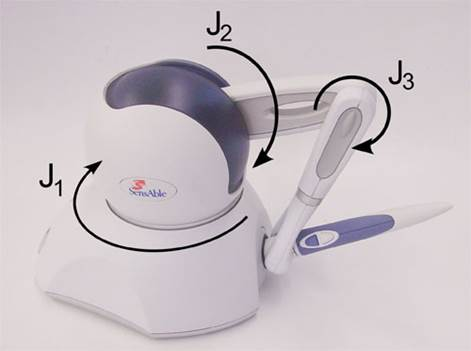
\includegraphics[width=\linewidth]{haptick1.jpg}
		\caption{Overview of the Phantom omni's first three joints.}
		\label{fig:phantom1}
	\end{subfigure}
	\begin{subfigure}{.45\textwidth}
		\centering
		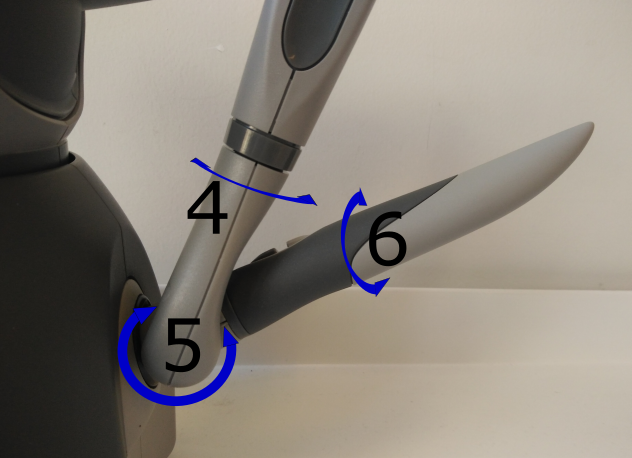
\includegraphics[width=\linewidth]{haptick2.png}
		\caption{Overview of the Phantom omni's last three joint}
		\label{fig:phantom2}
	\end{subfigure}
\caption{Overview of all the Phantom omni's joints\citep{phantom_omni}}
\label{fig:phantom_omni}
\end{figure}

As mentioned the Phantom omni has the ability to generate resistance for the user. In other words, when moved in a specific direction it can create a counter force in respect to a certain position. On \figref{fig:phantom_omni}, it can be seen that the omni has six \gls{DOF}, where the first three has actuators, see \figref{fig:phantom1}. This means that the device only has the ability to generate force feedback with three \gls{DOF}, in this case roll, pitch and yaw.

The connection to the omni can either be made directly through a ethernet cabel or through ethernet cabel to a usb converter into a computer. For programming the omni an API is included, which enables the connection to the omni. The programming of the omni happens through the languages C++. \todo{include other languages if any}

\subsection*{Installation of the Phantom omni}

The Phantom omni can be installed on both Windows, and Linux, embedded systems. 
Use the provided installation guides on\\
\url{http://dsc.sensable.com/viewforum.php?f=15}

\textbf{Note to the linux system:} If this installation is running on a non-US version of Linux, a readout of the different joint positions can be corrupted. This is because of the difference in the EU and US compiling, where the ',' and '.' is read different.\\
To solve this problem, follow the solution given on\\
\url{http://dsc.sensable.com/viewtopic.php?t=5644#top} \todo{This maby has to be set up every time}



% \begin{figure}[H]
% \centering
% \scalebox{1}{\input{rapport/pictures/phantom_omni.png}}
% \caption{Block diagram of the cascade.}
% \label{fig:RegBlock2}
% \end{figure}
